\documentclass[twocolumn,a4paper]{article}

\usepackage[landscape,left=2cm,right=2cm,top=1cm,bottom=1cm]{geometry}

\fboxrule=0.75pt
\setlength{\fboxsep}{0pt}
\setlength{\columnsep}{25pt}

\pagenumbering{gobble}

\usepackage[T1]{fontenc}
\usepackage[utf8]{inputenc}
\usepackage[swedish]{babel}
\usepackage{csquotes}
\usepackage{hyperref}
\usepackage{url}
\usepackage{graphicx}
\usepackage[flushleft]{threeparttable}
\usepackage{booktabs}
\usepackage{amsmath}
\usepackage{amssymb}
\usepackage{caption}

\begin{document}

%%%%%%%%%%%%%%%%%%%%%%%%%%%%%%%%%%%%%%%%%%%%%%%%%%%%%%%%%%%%%%%%%%%%%%%%%%%%%%%%%%%%%%%%%%%%%%%%%%%%%%%%%%%%%%%%%%%%%%%%%%%%%%%%%%%%%%%%%%%%
\section*{DNF solving}
För att lösa DNF uppgifter kan man skapa ett truth table med alla literaler som förekommer i uttrycket.
Sedan bygger man stegvis upp hela uttrycket med fler kolumner.
Se s.12 i Definitions för \emph{basic logic connectives}.
\begin{figure}[ht]
	\centering
	\fbox{\resizebox{0.85\columnwidth}{!}{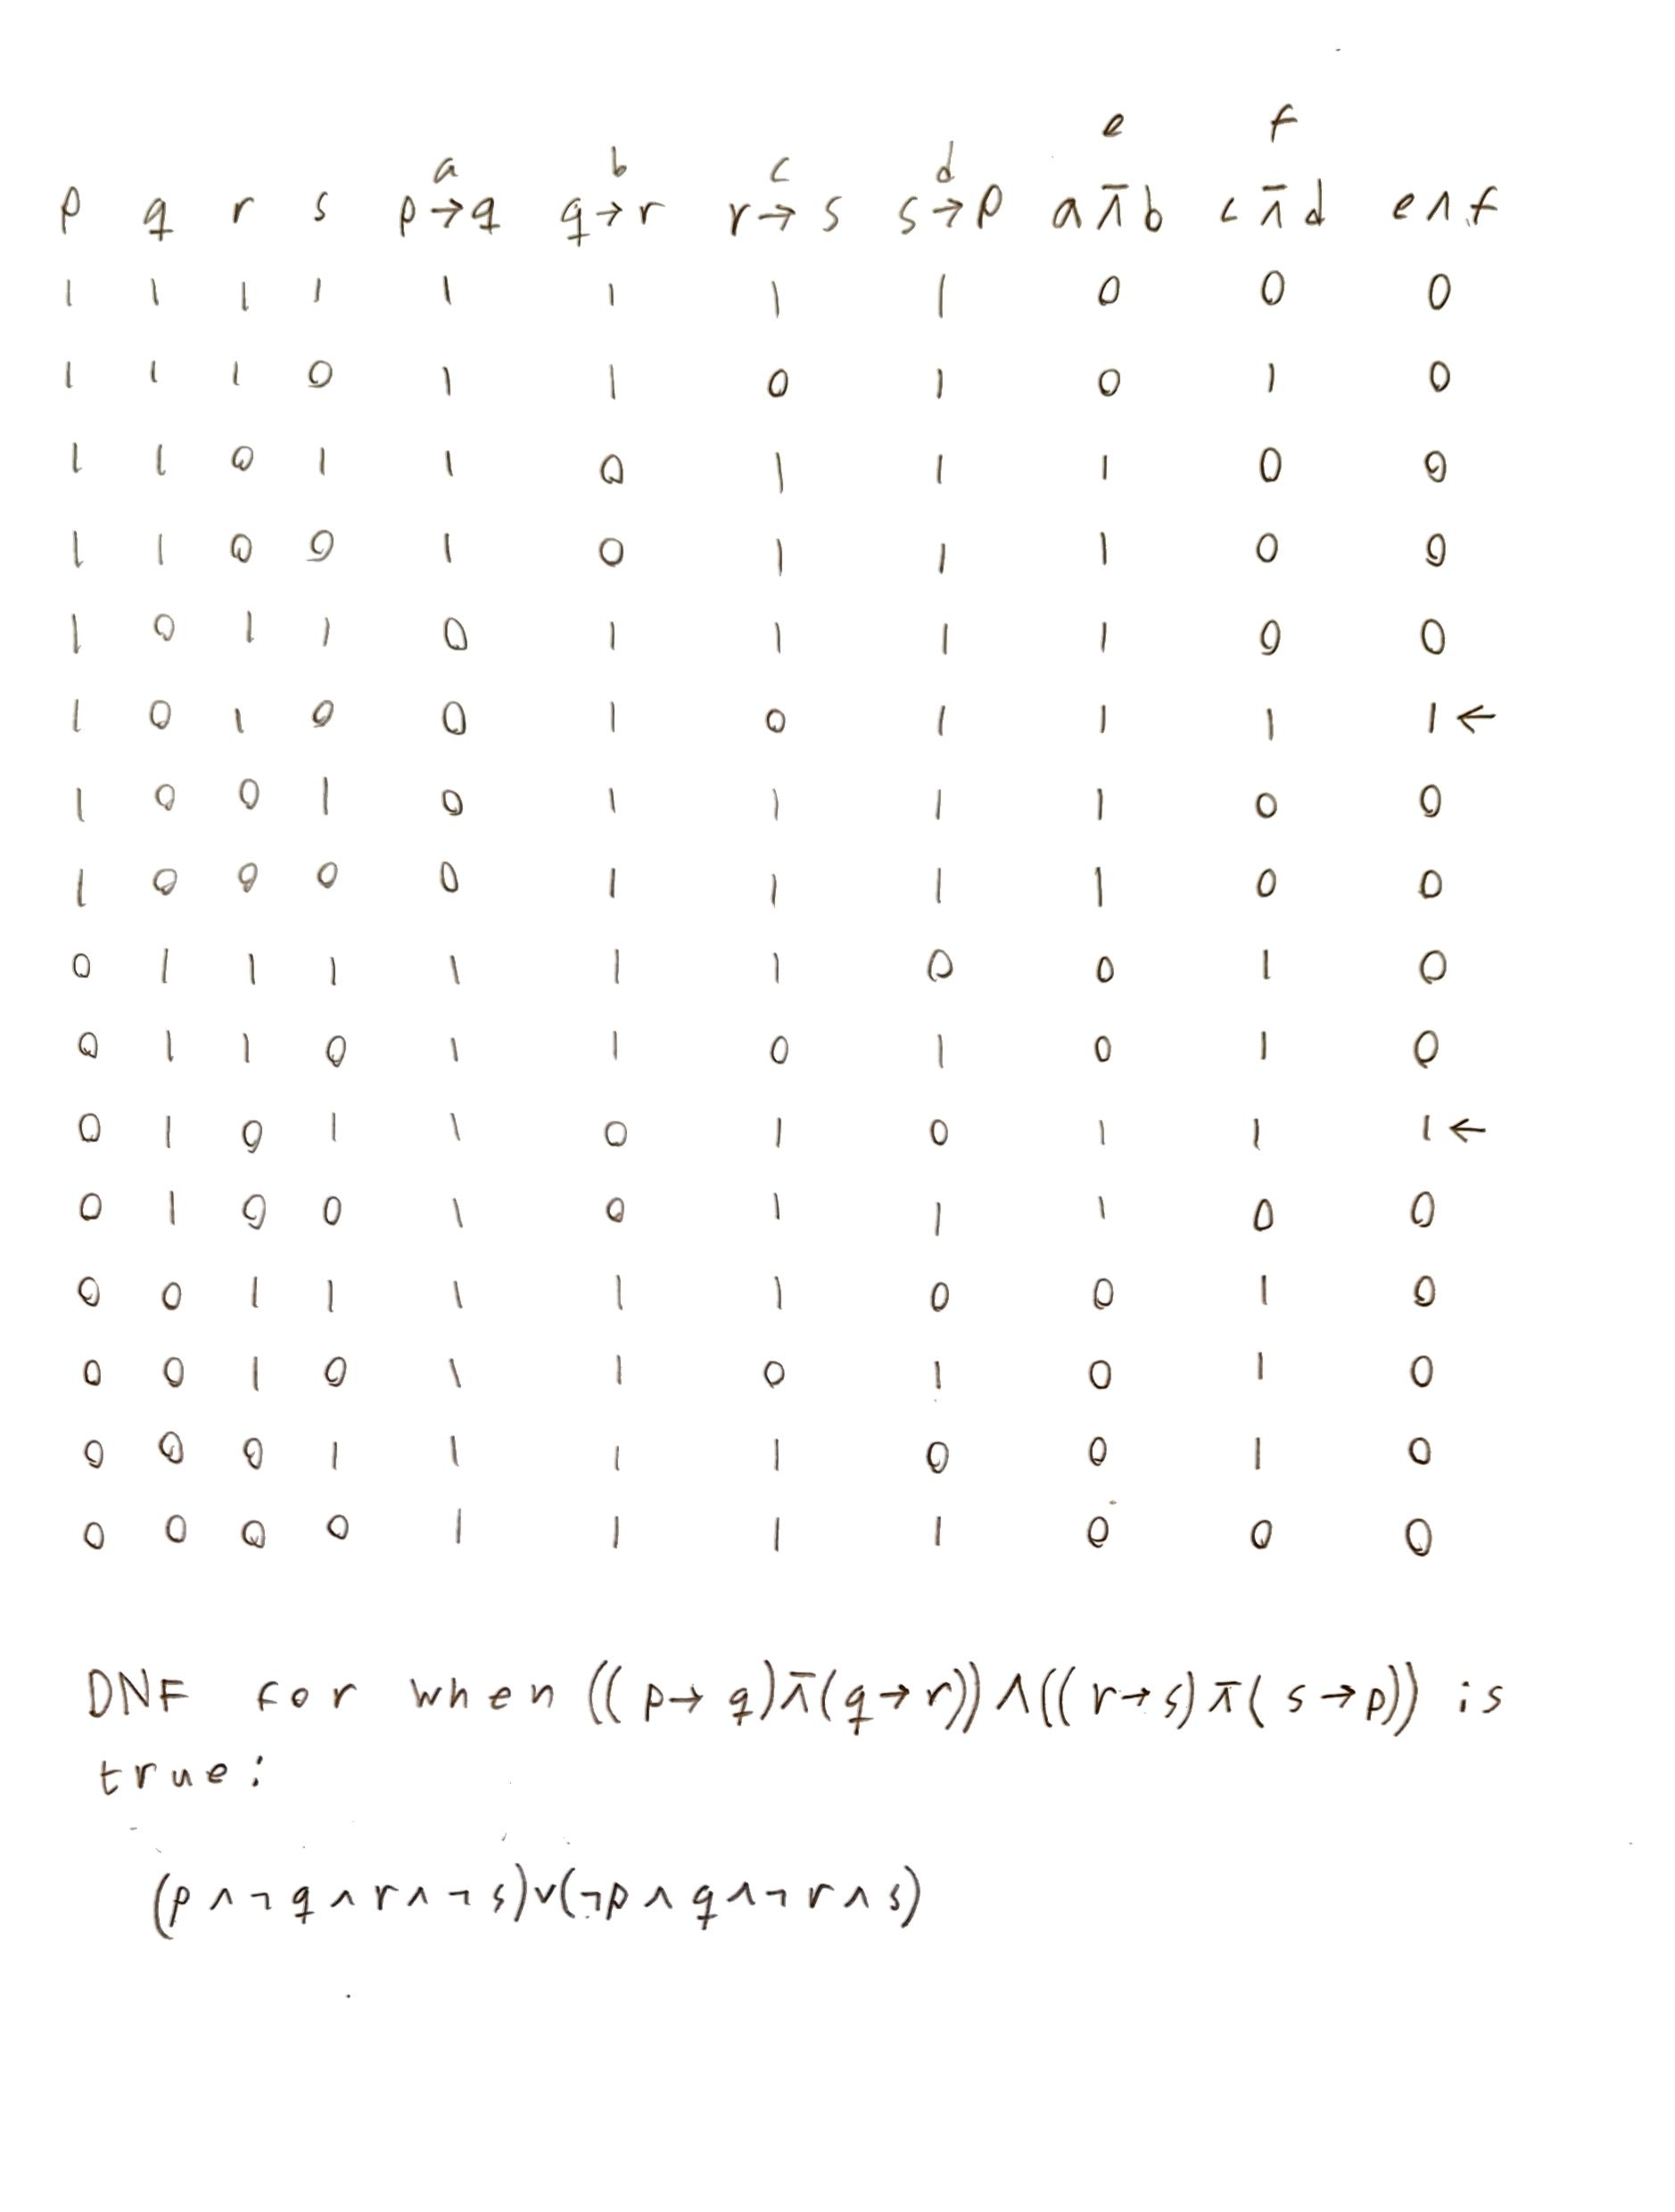
\includegraphics{2018_1/solution-5.1.jpeg}}}
\end{figure}

%%%%%%%%%%%%%%%%%%%%%%%%%%%%%%%%%%%%%%%%%%%%%%%%%%%%%%%%%%%%%%%%%%%%%%%%%%%%%%%%%%%%%%%%%%%%%%%%%%%%%%%%%%%%%%%%%%%%%%%%%%%%%%%%%%%%%%%%%%%%
\newpage
\section*{Intervals}

Here is a question about understanding how intervals change when sending through functions and meet.
TODO:\@ Understand answer and \([[]]\) syntax

\begin{figure}[ht]
	\centering
	\vspace{-10pt}
	\fbox{\resizebox{0.85\columnwidth}{!}{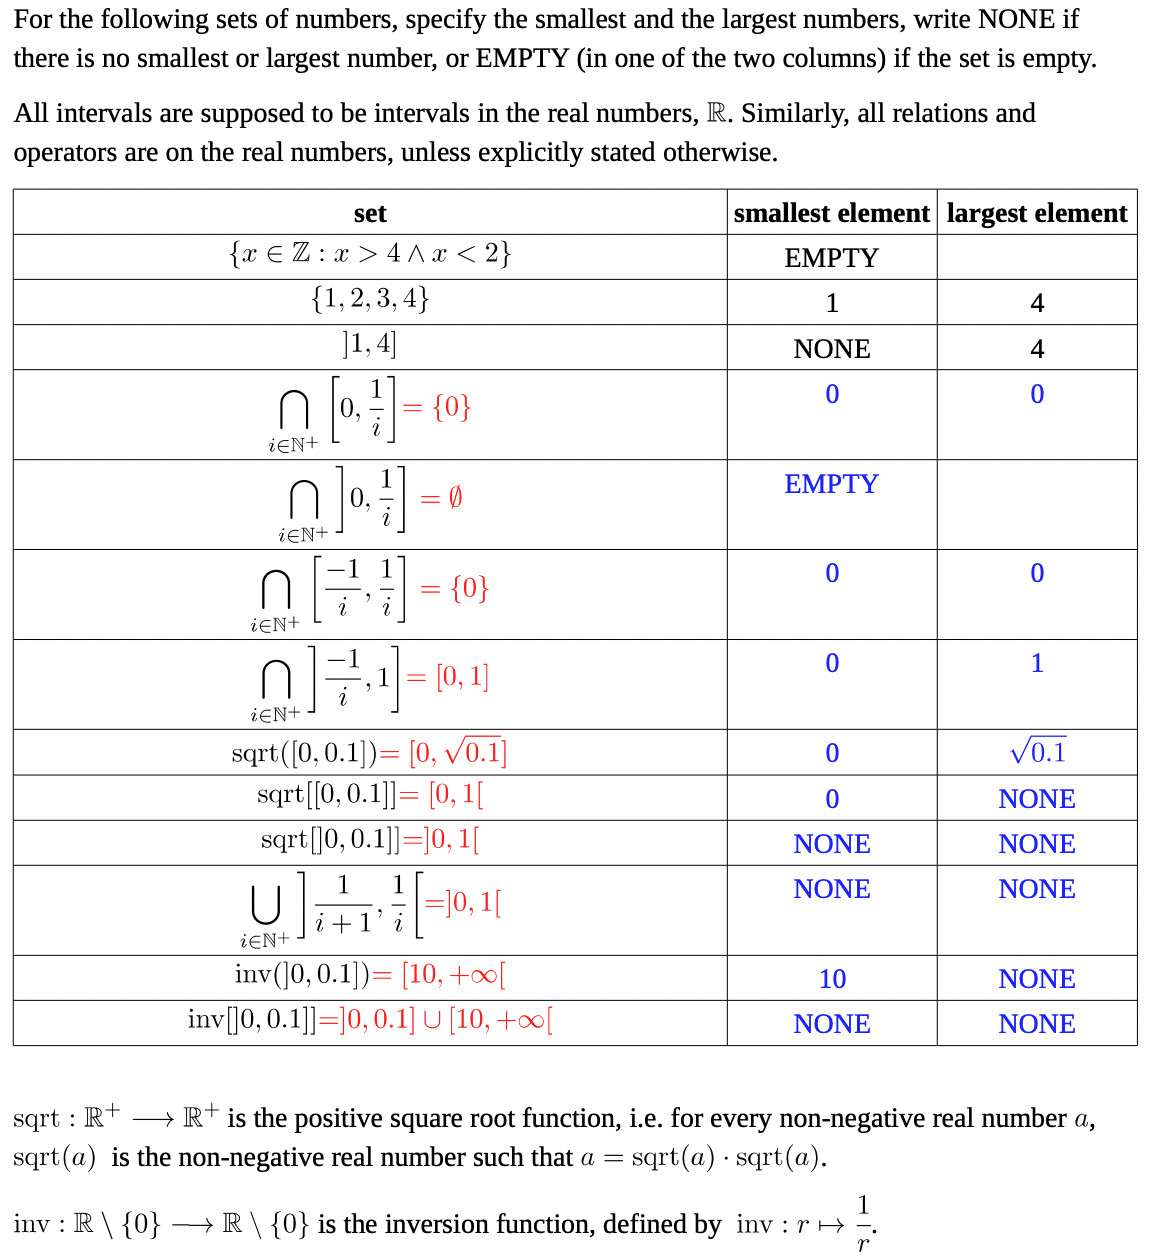
\includegraphics{2017_1/solution-1.png}}}
	\vspace{-10pt}
\end{figure}

Below is a explanation of how to think with intervals in more detail.
\begin{figure}[ht]
	\centering
	\vspace{-10pt}
	\fbox{\resizebox{0.85\columnwidth}{!}{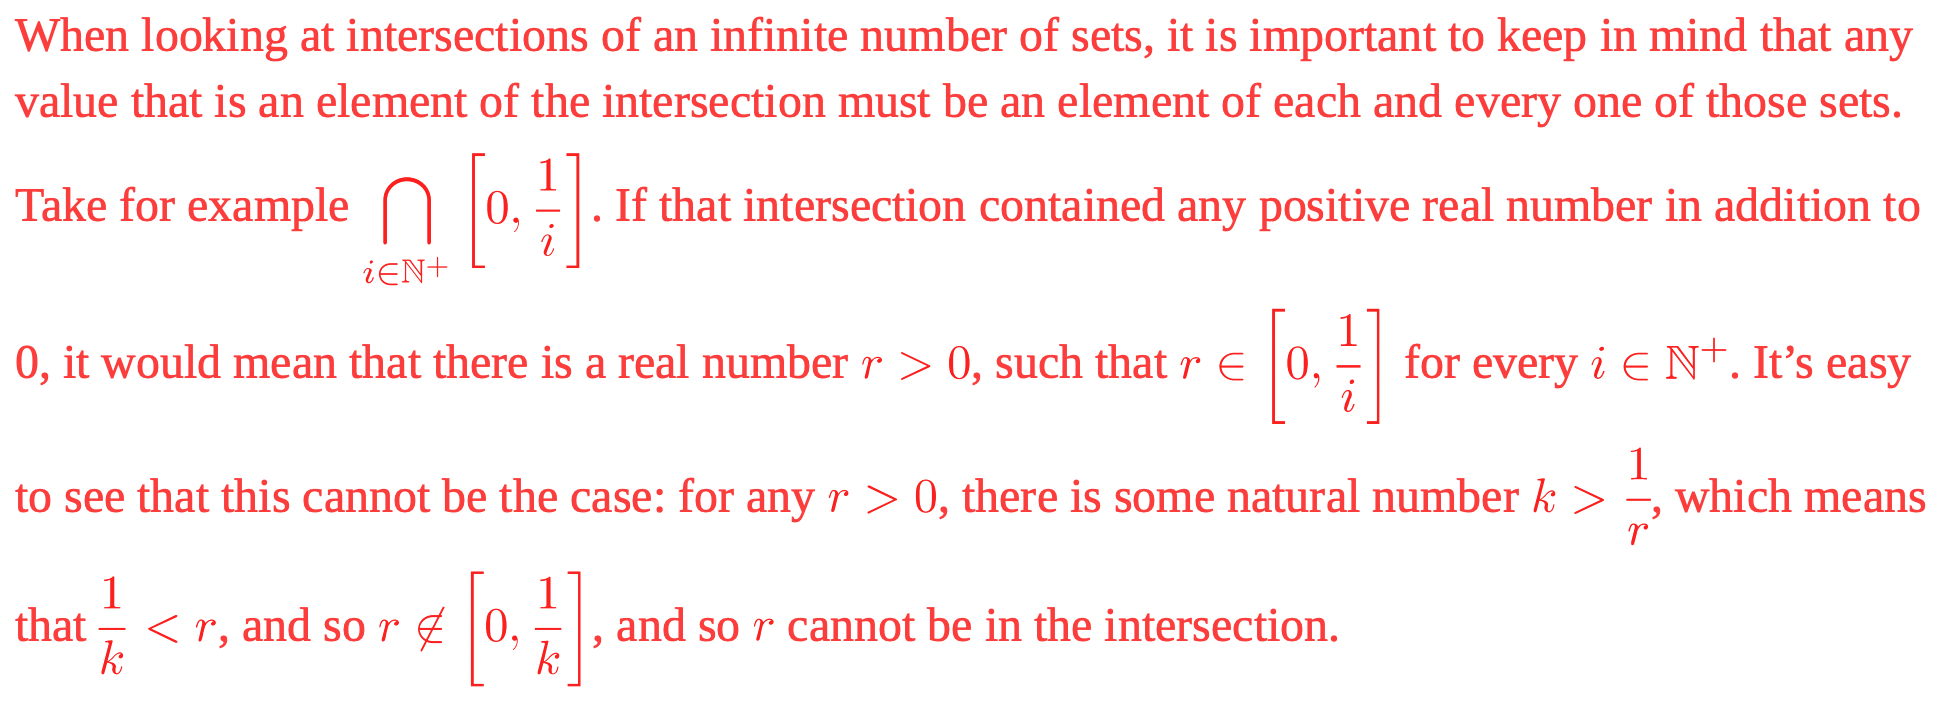
\includegraphics{2017_1/solution-1-explained.png}}}
	\vspace{-30pt}
\end{figure}

%%%%%%%%%%%%%%%%%%%%%%%%%%%%%%%%%%%%%%%%%%%%%%%%%%%%%%%%%%%%%%%%%%%%%%%%%%%%%%%%%%%%%%%%%%%%%%%%%%%%%%%%%%%%%%%%%%%%%%%%%%%%%%%%%%%%%%%%%%%%
\newpage
\section*{Injective and surjectiv}
This is an easier example for injective and surjective functions.
The reason why this question is easier is because we can define the domain and codomain seperatly.
\begin{figure}[ht]
	\centering
	\fbox{\resizebox{0.95\columnwidth}{!}{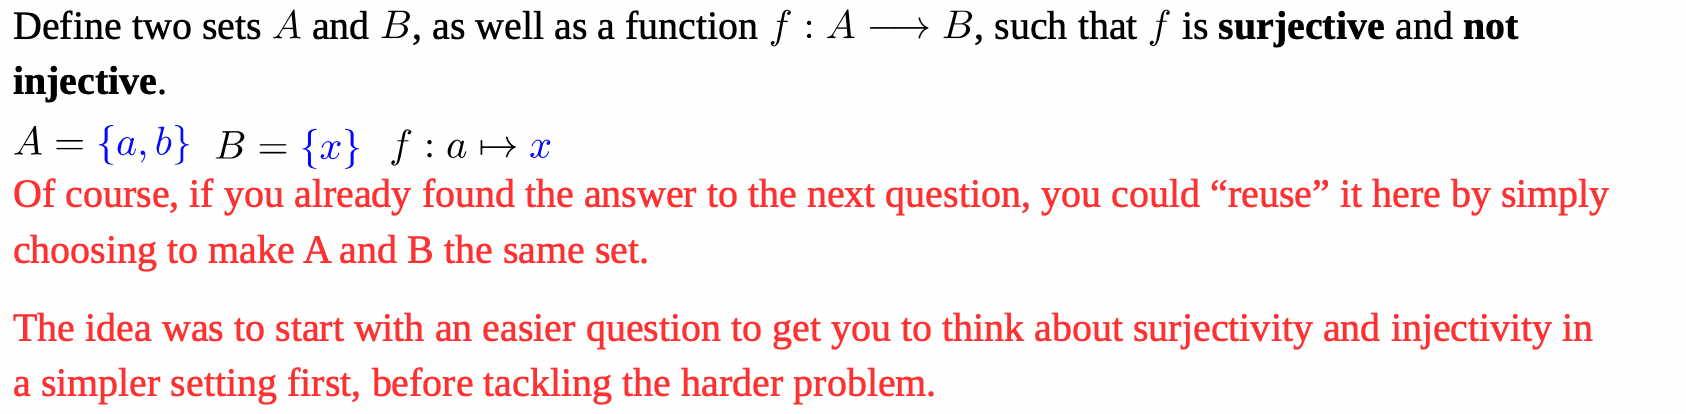
\includegraphics{2017_1/solution-2.png}}}
\end{figure}

With all of these weird example where something should be surjective and not injective and the codomain = domain we need to utilize infinte.
What is happening here is that any item in the codomain could be reached from the domain by takin the item plus one.
Meaning it is surjective but we also point to the same element twice.
\begin{figure}[ht]
	\centering
	\fbox{\resizebox{0.95\columnwidth}{!}{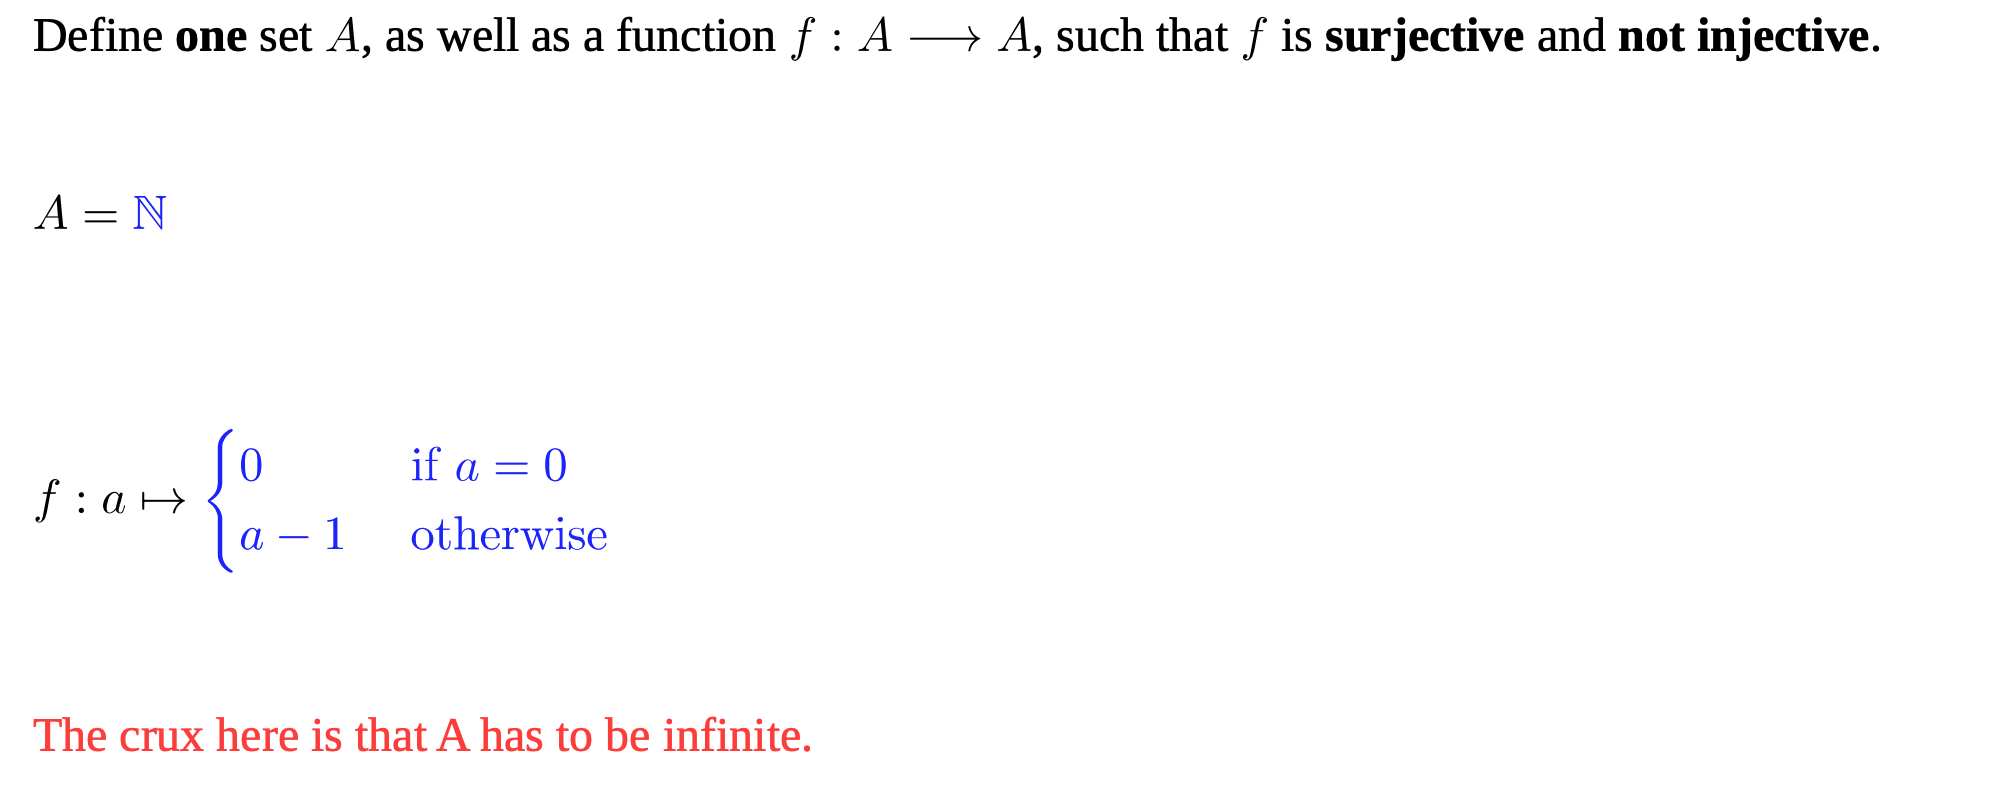
\includegraphics{2017_1/solution-3.png}}}
\end{figure}
\begin{figure}[ht]
	\centering
	\fbox{\resizebox{0.95\columnwidth}{!}{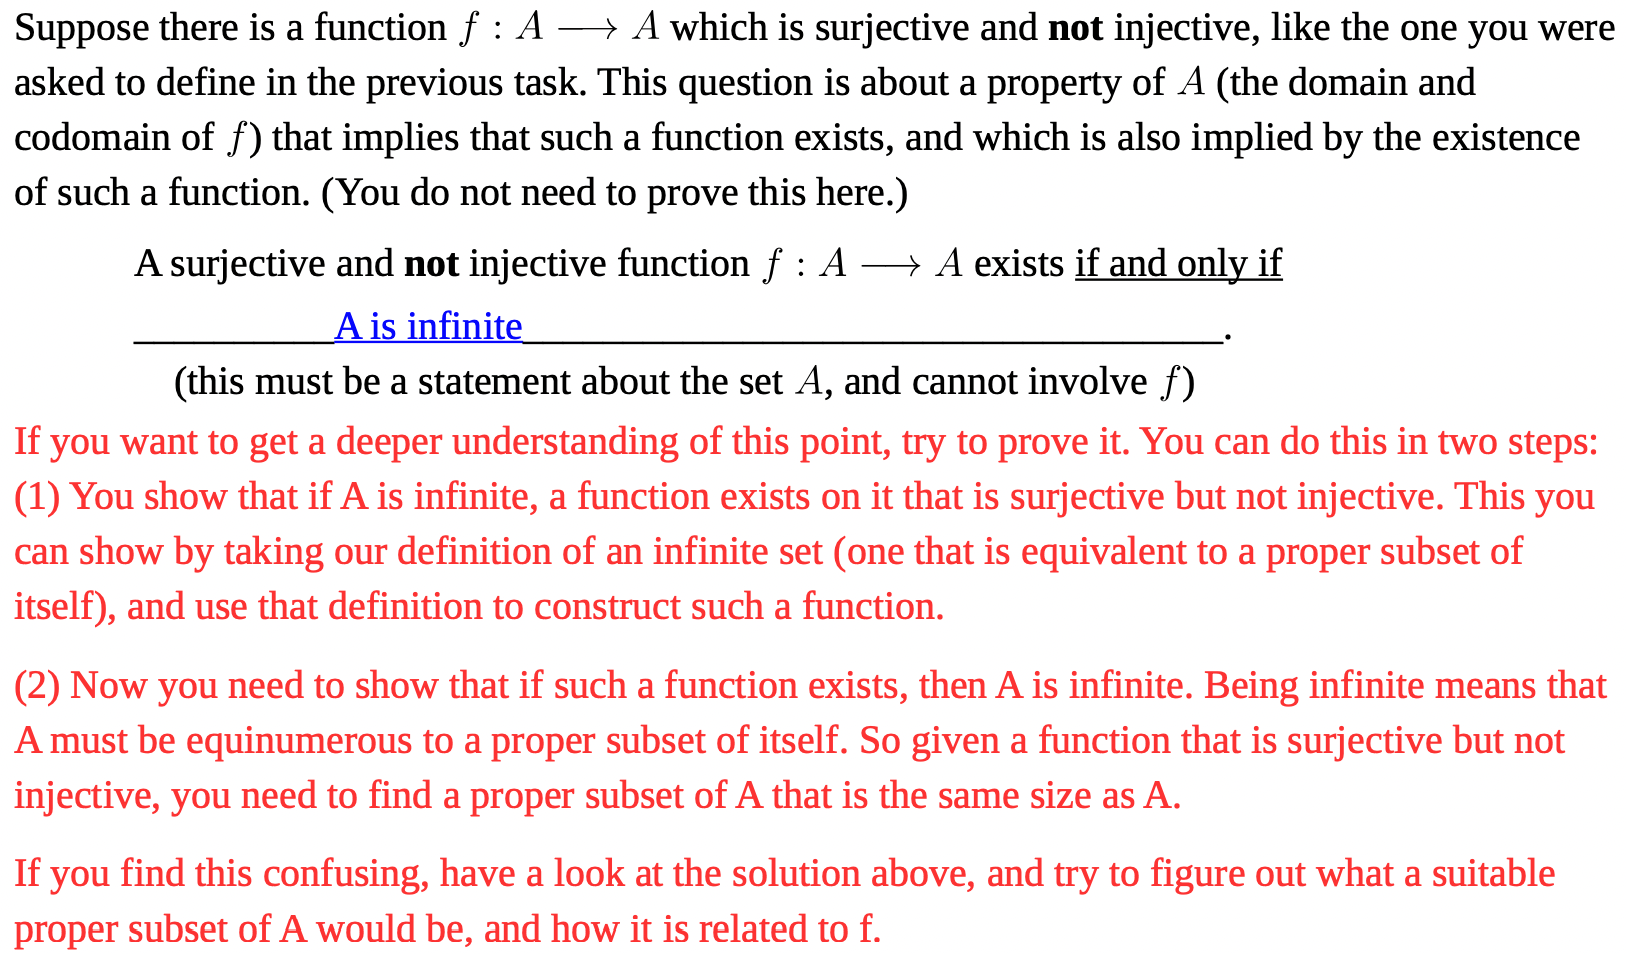
\includegraphics{2017_1/solution-4.png}}}
\end{figure}

%%%%%%%%%%%%%%%%%%%%%%%%%%%%%%%%%%%%%%%%%%%%%%%%%%%%%%%%%%%%%%%%%%%%%%%%%%%%%%%%%%%%%%%%%%%%%%%%%%%%%%%%%%%%%%%%%%%%%%%%%%%%%%%%%%%%%%%%%%%%
\newpage
\section*{Properties of paths, graphs and trees}
Here is an example of properties of an directed graph.
The interesting thing to remember is that no property is guaranteed.
We don't put any demands on our directed graph meaning it could be any kind of relation,
every node could be symmetric but then we would need to edges per node.
\begin{figure}[ht]
	\centering
	\fbox{\resizebox{0.95\columnwidth}{!}{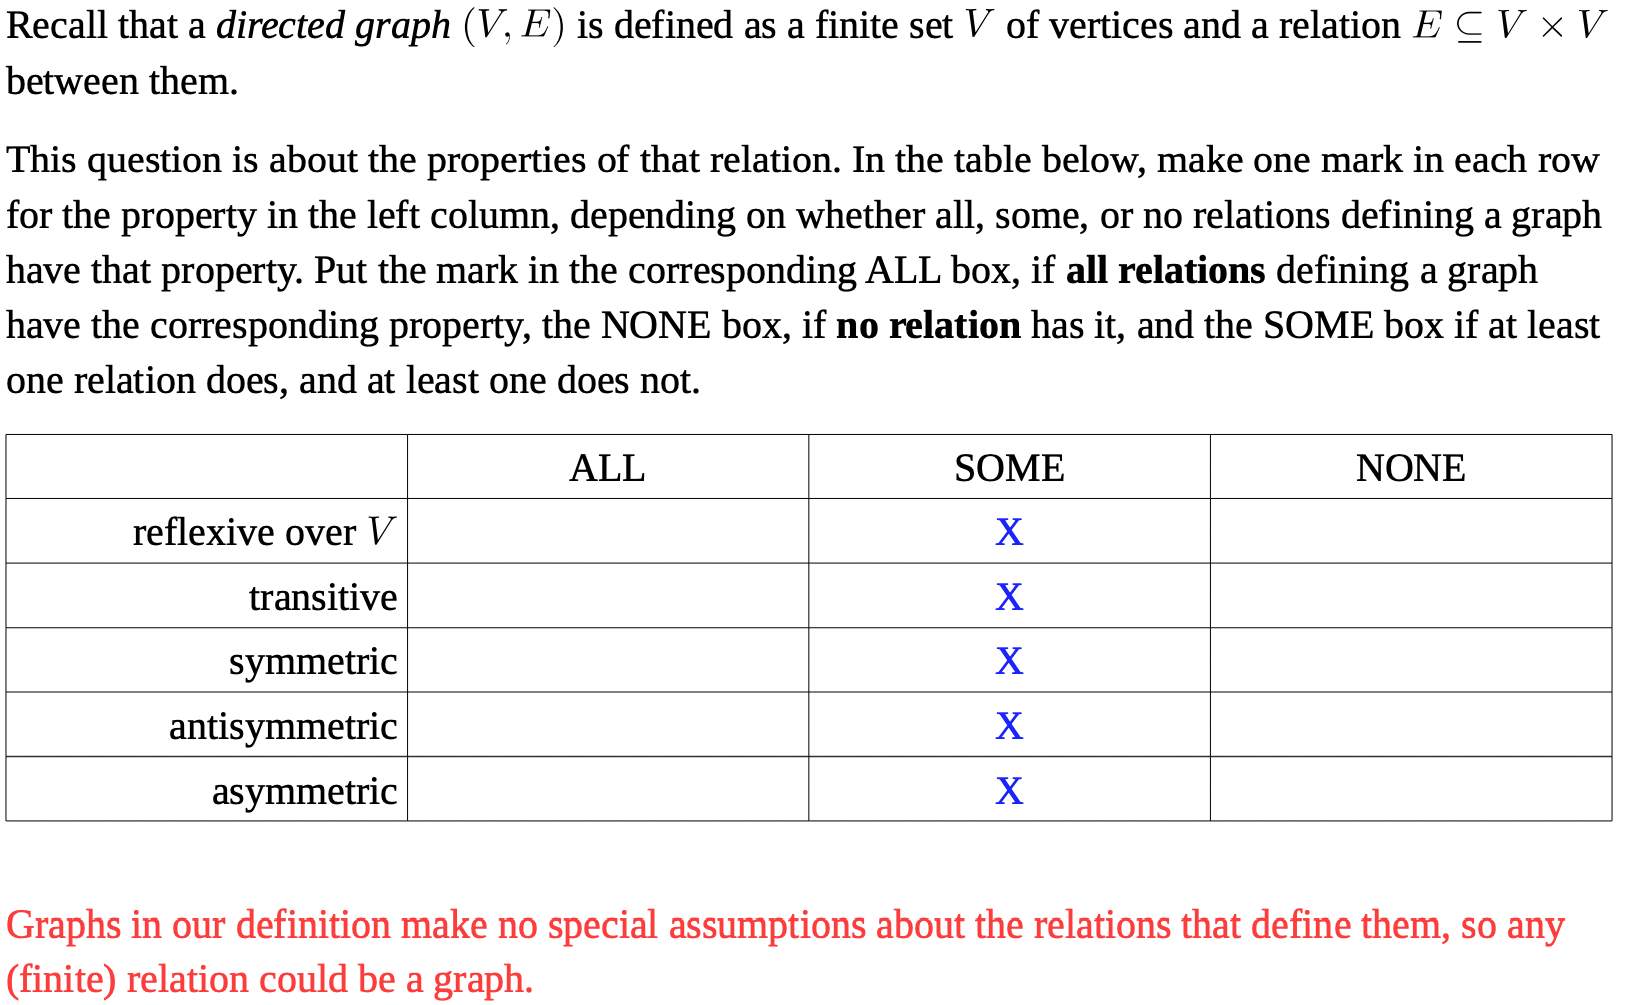
\includegraphics{2017_1/solution-5.png}}}
\end{figure}

This is an example of properties for a rooted tree.
This differs a bit from the example above, here some demands are put on the directed graph.
The reason why it is antisymmetric and asymetric is because if there exist (a,b) and (b,a) then there is a two ways to reach a,
you can go directly to be or go to a and then go to b and then a.
The reason why we don't allow antisymmetric is the same reason it is not reflexive.
\begin{figure}[ht]
	\centering
	\fbox{\resizebox{0.95\columnwidth}{!}{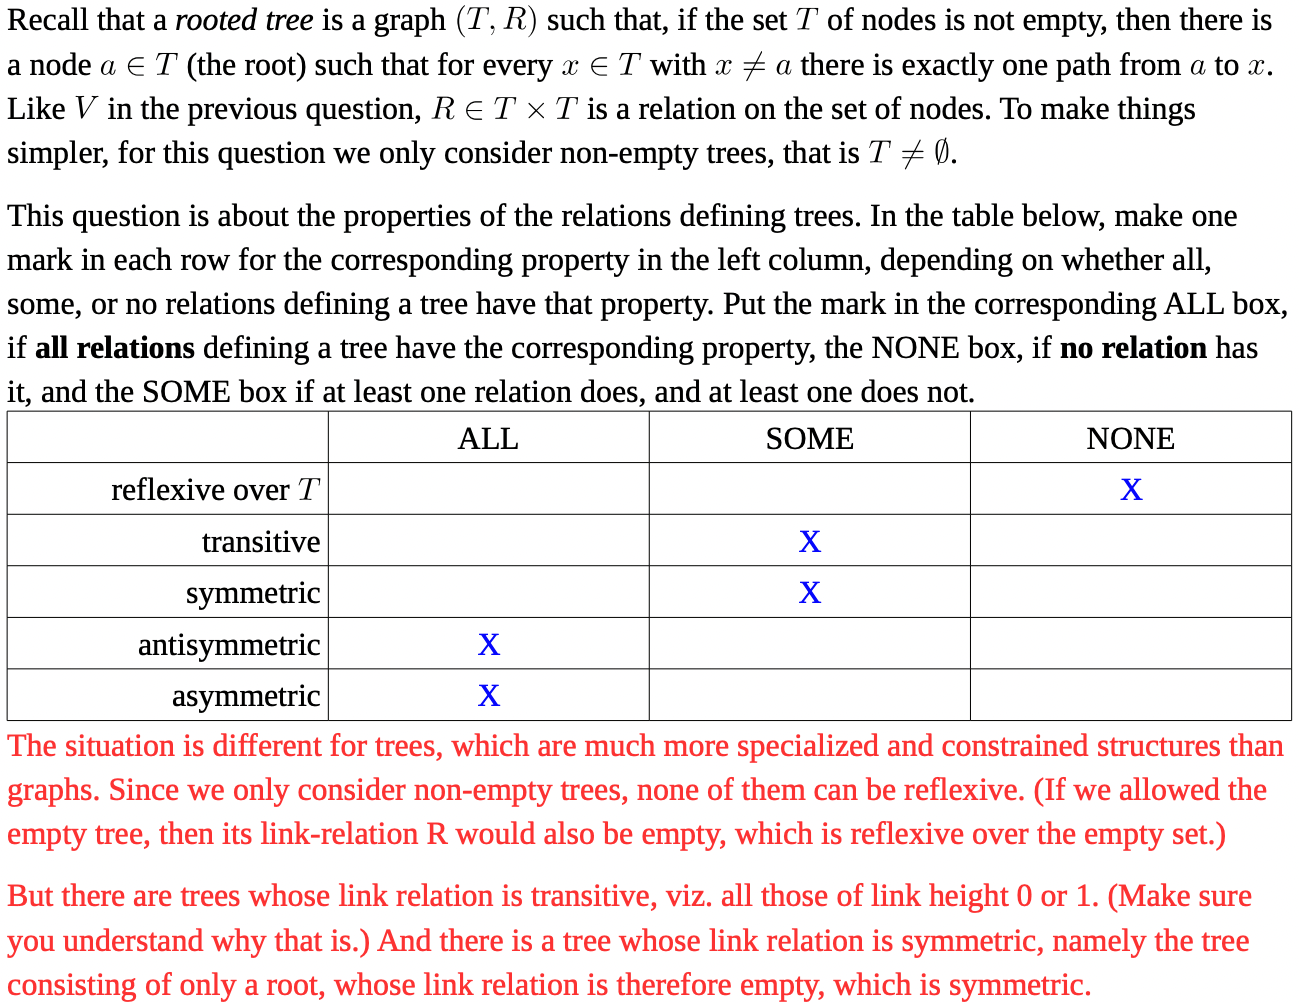
\includegraphics{2017_1/solution-6.png}}}
\end{figure}

%%%%%%%%%%%%%%%%%%%%%%%%%%%%%%%%%%%%%%%%%%%%%%%%%%%%%%%%%%%%%%%%%%%%%%%%%%%%%%%%%%%%%%%%%%%%%%%%%%%%%%%%%%%%%%%%%%%%%%%%%%%%%%%%%%%%%%%%%%%%
\newpage
\section*{Other important definitions}
\subsection*{Node height/depth}
The link-height (alias level) of a node in a tree is defined recursively: that of the root is 0,
and that of each of the children of a node is one greater than that of the node.
The node-height of a node (alias just its height in many texts) is defined by the same recursion,
except that the node-height of the root is set at 1.
Thus, for every node x, \(node-height(x) = link-height(x) + 1\).
As trees are usually drawn upside-down, the term `depth' is often used instead of `height'.

\subsection{CNF}
Conjunctive normal form is like disjunctive normal form but ‘upside-down’: the roles of disjunction and conjunction are reversed. 
A basic disjunction is defined to be any disjunction of (one or more) literals in which no letter occurs more than once.
A formula is said to be in conjunctive normal form (cnf) iff it is a conjunction of (one or more) basic disjunctions

\subsection*{Edge cases for always/sometimes/never problems}
If you have a graph \((V, E)\), then you should check the edge cases where:
\begin{enumerate}
	\item \(V=\emptyset \) or \(E=\emptyset \).
	\item \(V\) only contains 1 node or 2 nodes.
	\item \(E\) contains a connection in one direction but not back. And when it contains a connection in both directions.
	\item All nodes are connected to all nodes.
\end{enumerate}

\subsection*{Quantifiers}

\(\forall x\in\emptyset(\ldots) = true\). \\
\(\exists x\in\emptyset(\ldots) = false\).

\subsection*{Logic operators}
\begin{enumerate}
	\item $\alpha \barwedge \beta = \neg (\alpha \wedge \beta)$ and $\neg \alpha = (\alpha \barwedge \alpha)$
\end{enumerate}

\subsection*{Image of n-ary}
When computing the imager, we treat the last position of a relation as its `output`. 
\begin{equation}
	R(a_1, \ldots, a_{n-1}) = \{a \in A : (a_1, \ldots, a_{n-1}, a) \in R \}
\end{equation}
\end{document}